\documentclass{jsarticle}
\usepackage[top=20truemm,bottom=20truemm,left=25truemm,right=25truemm]{geometry}
\usepackage{amsmath,ascmac,url,amsfonts,bm,here,algorithmic,algorithm,amsthm,color}
\usepackage[dvipdfmx]{graphicx}
\newcommand{\argmax}{\mathop{\rm argmax}\limits}
\newcommand{\argmin}{\mathop{\rm argmin}\limits} 
\newcommand{\expect}{\mathbb{E}} 
\newcommand{\trans}[1]{#1^{\top}}
\newcommand{\pdif}[2]{\frac{\partial#1}{\partial#2}}
\newcommand{\odif}[2]{\frac{\rm{d}#1}{\rm{d}#2}}
\makeatletter
  \def\@maketitle{
  \newpage\null
  \vskip 2em
    \mbox{}\hfill
    \begin{flushleft}
    \textbf{制御システム論分野研究会資料}
    \end{flushleft}
    \begin{flushright}
    {\lineskip .5em
      \begin{tabular}[t]{c}
        \@date \\
        \@author
      \end{tabular}\par}
        \end{flushright}
  \begin{center}
  \let\footnote\thanks
    {\LARGE \@title \par}
    \vskip 1.5em
  \end{center}
    \vskip 1em
  \par}
\makeatother
\title{\large{\bf{進捗報告 8.28}}}
\author{M2 竹内 維吹}
%\date{Jul. 7, 2020}
\date{\today}
\begin{document}
\maketitle


\section{サンプル値系システムの強化学習}
対象のシステムが
\begin{equation}
	s_{t+1} = f(s_t) + g(s_t)a_t
\end{equation}
と書かれていて,  $\tau$ステップ毎に状態を観測し, 状態フィードバック制御則を変えて次の観測までは同じ入力を加え続ける, サンプル値系における最適制御問題の強化学習を考える. この動機は$\tau$ステップ毎に観測・制御則更新を行うのと, それを毎ステップ行う(以下, 毎時刻系と呼ぶ)のとで学習に必要なステップ数が変わるのかを検証するためである.\par
結論から記すと, サンプル値系にすると学習時間が増えることが確認できた. 
% 1ステップとサンプル値系で同じような制御性能に至るまでに必要なステップをそれぞれ探す

\subsection{倒立振子による実験}
倒立時の振子の角度を$\theta=0$とし, 加えられる入力が$A=[-10\textrm{N}\cdot\textrm{m},10\textrm{N}\cdot\textrm{m}]$と制限されるような倒立振子を考える.この倒立振子のダイナミクスは, 以下のように与えられる.
\begin{align}
	\theta_{t+1} &= \theta_t+\dot{\theta}_t\delta_t+\frac{3g}{2l}\sin{\theta_t}\delta_t^2+\frac{3}{ml^2}a\delta_t^2 \\
	\dot{\theta}_{t+1} &=  \dot{\theta}_t+\frac{3g}{2l}\sin{\theta_t}\delta_t+\frac{3}{ml^2}a\delta_t
\end{align}
ただし, $\delta_t$は離散化定数であり$\delta_t=0.05$とする.\par

\subsection{エピソード間蓄積報酬による検証}
毎時刻系とサンプル値系の強化学習に必要なステップ数を確認するために, 方策の変化とエピソード報酬の変化の関係を見る. ただしエピソードとは, 200ステップの離散システムの動作を1まとまりにしたものとする. 「環境とのインタラクション」という言葉を「状態変数・即時報酬の観測と, 新たな入力信号をアクチュエータに送信すること」と定義すると,  $\tau=5$のサンプル値系では1エピソードの間に40回のインタラクションを行う事になる. 1回のインタラクションにつき, 1回制御則を更新することに注意されたい. \par
では, 毎時刻系とサンプル値系の学習におけるエピソード報酬の変化を確認していく. 
\begin{figure}[h]
	\centering
 	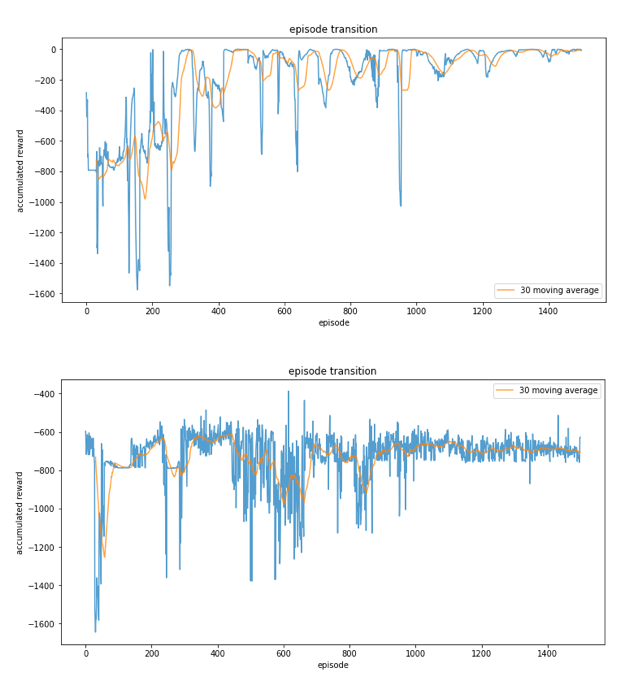
\includegraphics[width=12cm]{episode_reward.png} \label{episode_reward}
 	\caption{毎時刻系とサンプル値系のエピソード報酬}
\end{figure}\\
図1の上段が毎時刻系, 下段がサンプル値系をそれぞれ表す. これらのグラフの横軸はエピソード数を表しているので, 当然ステップ数も同じである. しかしながら毎時刻系とサンプル値系では「インタラクション」の回数が異なるため, $\tau=5$のサンプル値系では毎時刻系に対してインタラクション回数は, 毎時刻系の$\frac{1}{5}$となる. これを見ると毎時刻系では1200エピソード付近で最適に近い制御則が学習できていることが確認できるが, サンプル値系では「まだ」改善はみられていない. これはサンプル値系にすると必要なステップ数が増えることの証左となる.\newpage
では毎時刻系で得られているエピソード報酬を得られる制御則を, サンプル値系でも学習するにはどのくらいのエピソードが必要なのか, この学習の続きを見ていく.
\begin{figure}[h]
	\centering
 	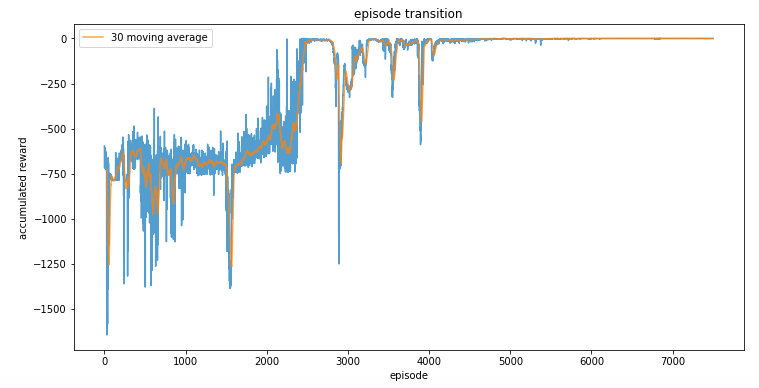
\includegraphics[width=12cm]{sample_value.png} \label{sample_value}
 	\caption{サンプル値系のさらなる学習}
\end{figure}\\
図2を見ると, 4000エピソード付近で最適制御則を学習できていることがわかる. これは毎時刻系の約3倍であり, $\tau=5$よりも小さな値であるため, 1回の制御則更新の効率は毎時刻系よりも$\frac{5}{3}$倍程度良くなっていることがわかる. したがって, システムの1ステップの時間発展の計算にかかる時間が, ニューラルネットワークのパラメータ更新にかかる計算時間よりも十分に小さい計算機上では, ステップ数が増えてしまうことは大きな脅威とはならないかもしれない.\par
(しかしこれは1回の学習から得られた考察なので, より強く断定するには少し学習タスクのサンプル数を増やす必要がある.)

\section{セルフトリガー制御にむけて}
強化学習エージェントは制御則$\pi(s)$を$\pi_{\theta}(s)$のようにパラメトライズし, その最適パラメータを模索する. ここでは, 毎時刻系の最適エージェントのパラメータを初期値として, サンプル間隔$\tau$を変えた時に制御性能を満たすことを学習できるのかどうか検証したい. 

\subsection{毎時刻系の最適エージェント}
方策$\pi_{\theta}(s)$は以下のようなニューラルネットワークモデルを用いる. 

\begin{figure}[h]
	\centering
 	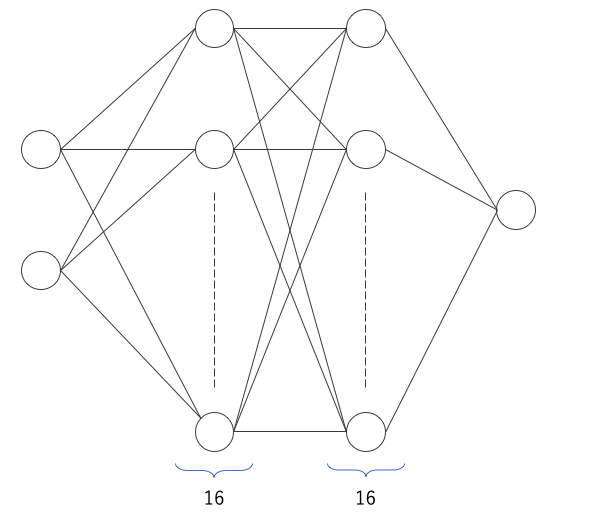
\includegraphics[width=8cm]{actor.png} 
 	\caption{方策$\pi(s)$の表現モデル}
\end{figure}

この時各層の一部のニューロンの活性化関数を線形関数$y=x$にして, 重みを適切に設定してやることで線形フィードバック制御則を実現することが可能である. 毎時刻系で原点付近を安定化させる方策を初期値として,  $\tau$を変えても原点付近の安定化方策の学習ができるか試みた.\par
いま, 図3の出力層の活性化関数も線形関数としているが, こうしてしまうと値域が$(-\infty, \infty)$となってしまう. これは入力信号に制限がある場合には不都合がある.
例えば入力制限を$[-10, 10]$とし, これ以外の入力を加えようとした場合, 制限集合の最も近い入力がシステムに加わるとする. 現在用いているDDPGアルゴリズムはactor-critic構造となっており, critic側の損失が非常に重要である. criticの損失関数にはTD誤差を用いたものが使用されている. ここでいうTD誤差とは
\begin{equation}
	\delta_{TD} = Q(s_t, a_t) - \{r_t + \gamma Q(s_{t+1}, \pi(s_{t+1}))\}
\end{equation}
である.\par

今, criticの損失関数の値が発散してしまうと言う問題点が発生しています.(おそらくはこれは, $\pi(s)$の出力と実際にシステムに加えられる入力が異なることによって, TD誤差が発散していることだろうと考えていますが, なぜそうなるのかわかっていません.)\par

出力層の活性化関数を$\tanh$のスカラー倍にすることで, 予想している原因を回避できるがこれでは毎時刻系の最適エージェントをニューラルネットワークモデルとして設計することができない. よって模倣学習を用いるか, 毎時刻系エージェントを強化学習によって得るかする必要がある.


 
\end{document}